\chapter{METODE PENELITIAN}

\section{Jenis Penelitian}
Penelitian ini melakukan deteksi objek pada data citra dermoskopi menggunakan metode YOLO-v7. Berdasarkan hal tersebut, penelitian ini data numerik yang terdiri dari matriks dan nilai intensitas piksel sehingga penelitian ini termasuk ke dalam penelitian kuantitatif. Maka dari itu, pada penelitian ini terdapat perhitungan dan analisis terkait dengan data dan metode yang digunakan untuk mendeteksi kanker kulit pada citra dermoskopi.

\section{Jenis dan Sumber Data}
Penelitian ini menggunakan dataset yang berasal dari \textit{ISIC 2019 Challenge}. Dataset \textit{ISIC 2019 Challenge} memiliki 8 jenis kanker kulit, yaitu \textit{Actinic Keratosis}, \textit{Melanoma}, \textit{Squamous Cell Carcinoma}, \textit{Basal Cell Carcinoma}, \textit{Nevus}, \textit{Dermatofibroma}, \textit{Benign Keratosis Lesion}, dan \textit{Vascular Lesion}. Terdapat ribuan data citra kanker kulit, akan tetapi dengan mempertimbangkan perangkat yang digunakan untuk pembentukan model, penelitian ini menggunakan 200 citra pada tiap kelas sehingga terdapat 1600 data citra yang digunakan pada penelitian ini untuk pembentukan model. Sampel citra masing-masing jenis kanker kulit seperti terlihat pada Gambar \ref{fig:dataset}.

\begin{figure}[H]
    \centering
    \begin{tabular}{cccc}
        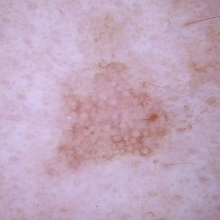
\includegraphics[width=2cm]{../img/Dataset - AK.png}
        &
        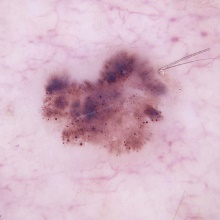
\includegraphics[width=2cm]{../img/Dataset - BCC.png}
        &
        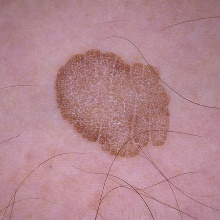
\includegraphics[width=2cm]{../img/Dataset - BKL.png}
        &
        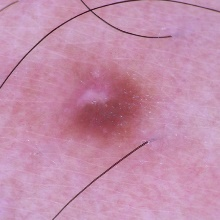
\includegraphics[width=2cm]{../img/Dataset - DF.png}\\
        (a) &(b) &(c) &(d)\\
        \  &\  &\  &\ \\
        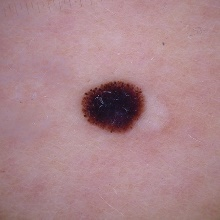
\includegraphics[width=2cm]{../img/Dataset - MEL.png}
        &
        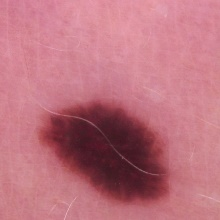
\includegraphics[width=2cm]{../img/Dataset - NV.png}
        &
        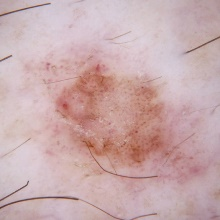
\includegraphics[width=2cm]{../img/Dataset - SCC.png}
        &
        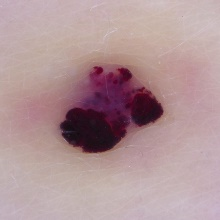
\includegraphics[width=2cm]{../img/Dataset - VASC.png}\\
        (e) &(f) &(g) &(h)\\
    \end{tabular}
    \caption{Dataset citra dermoskopi kanker kulit (a) AK; (b) BCC; (c) BKL; (d) DF; (e) MEL; (f) NV; (g) SCC; (h) VASC;}
    \label{fig:dataset}
\end{figure}

\section{Kerangka Penelitian}
Tahapan dalam melakukan deteksi kanker kulit berdasarkan citra dermoskopi menggunakan YOLO-v7 pada penelitian ini seperti terlihat pada Gambar \ref{fig:flowchart}.

\begin{figure}[H]
    \begin{center}
        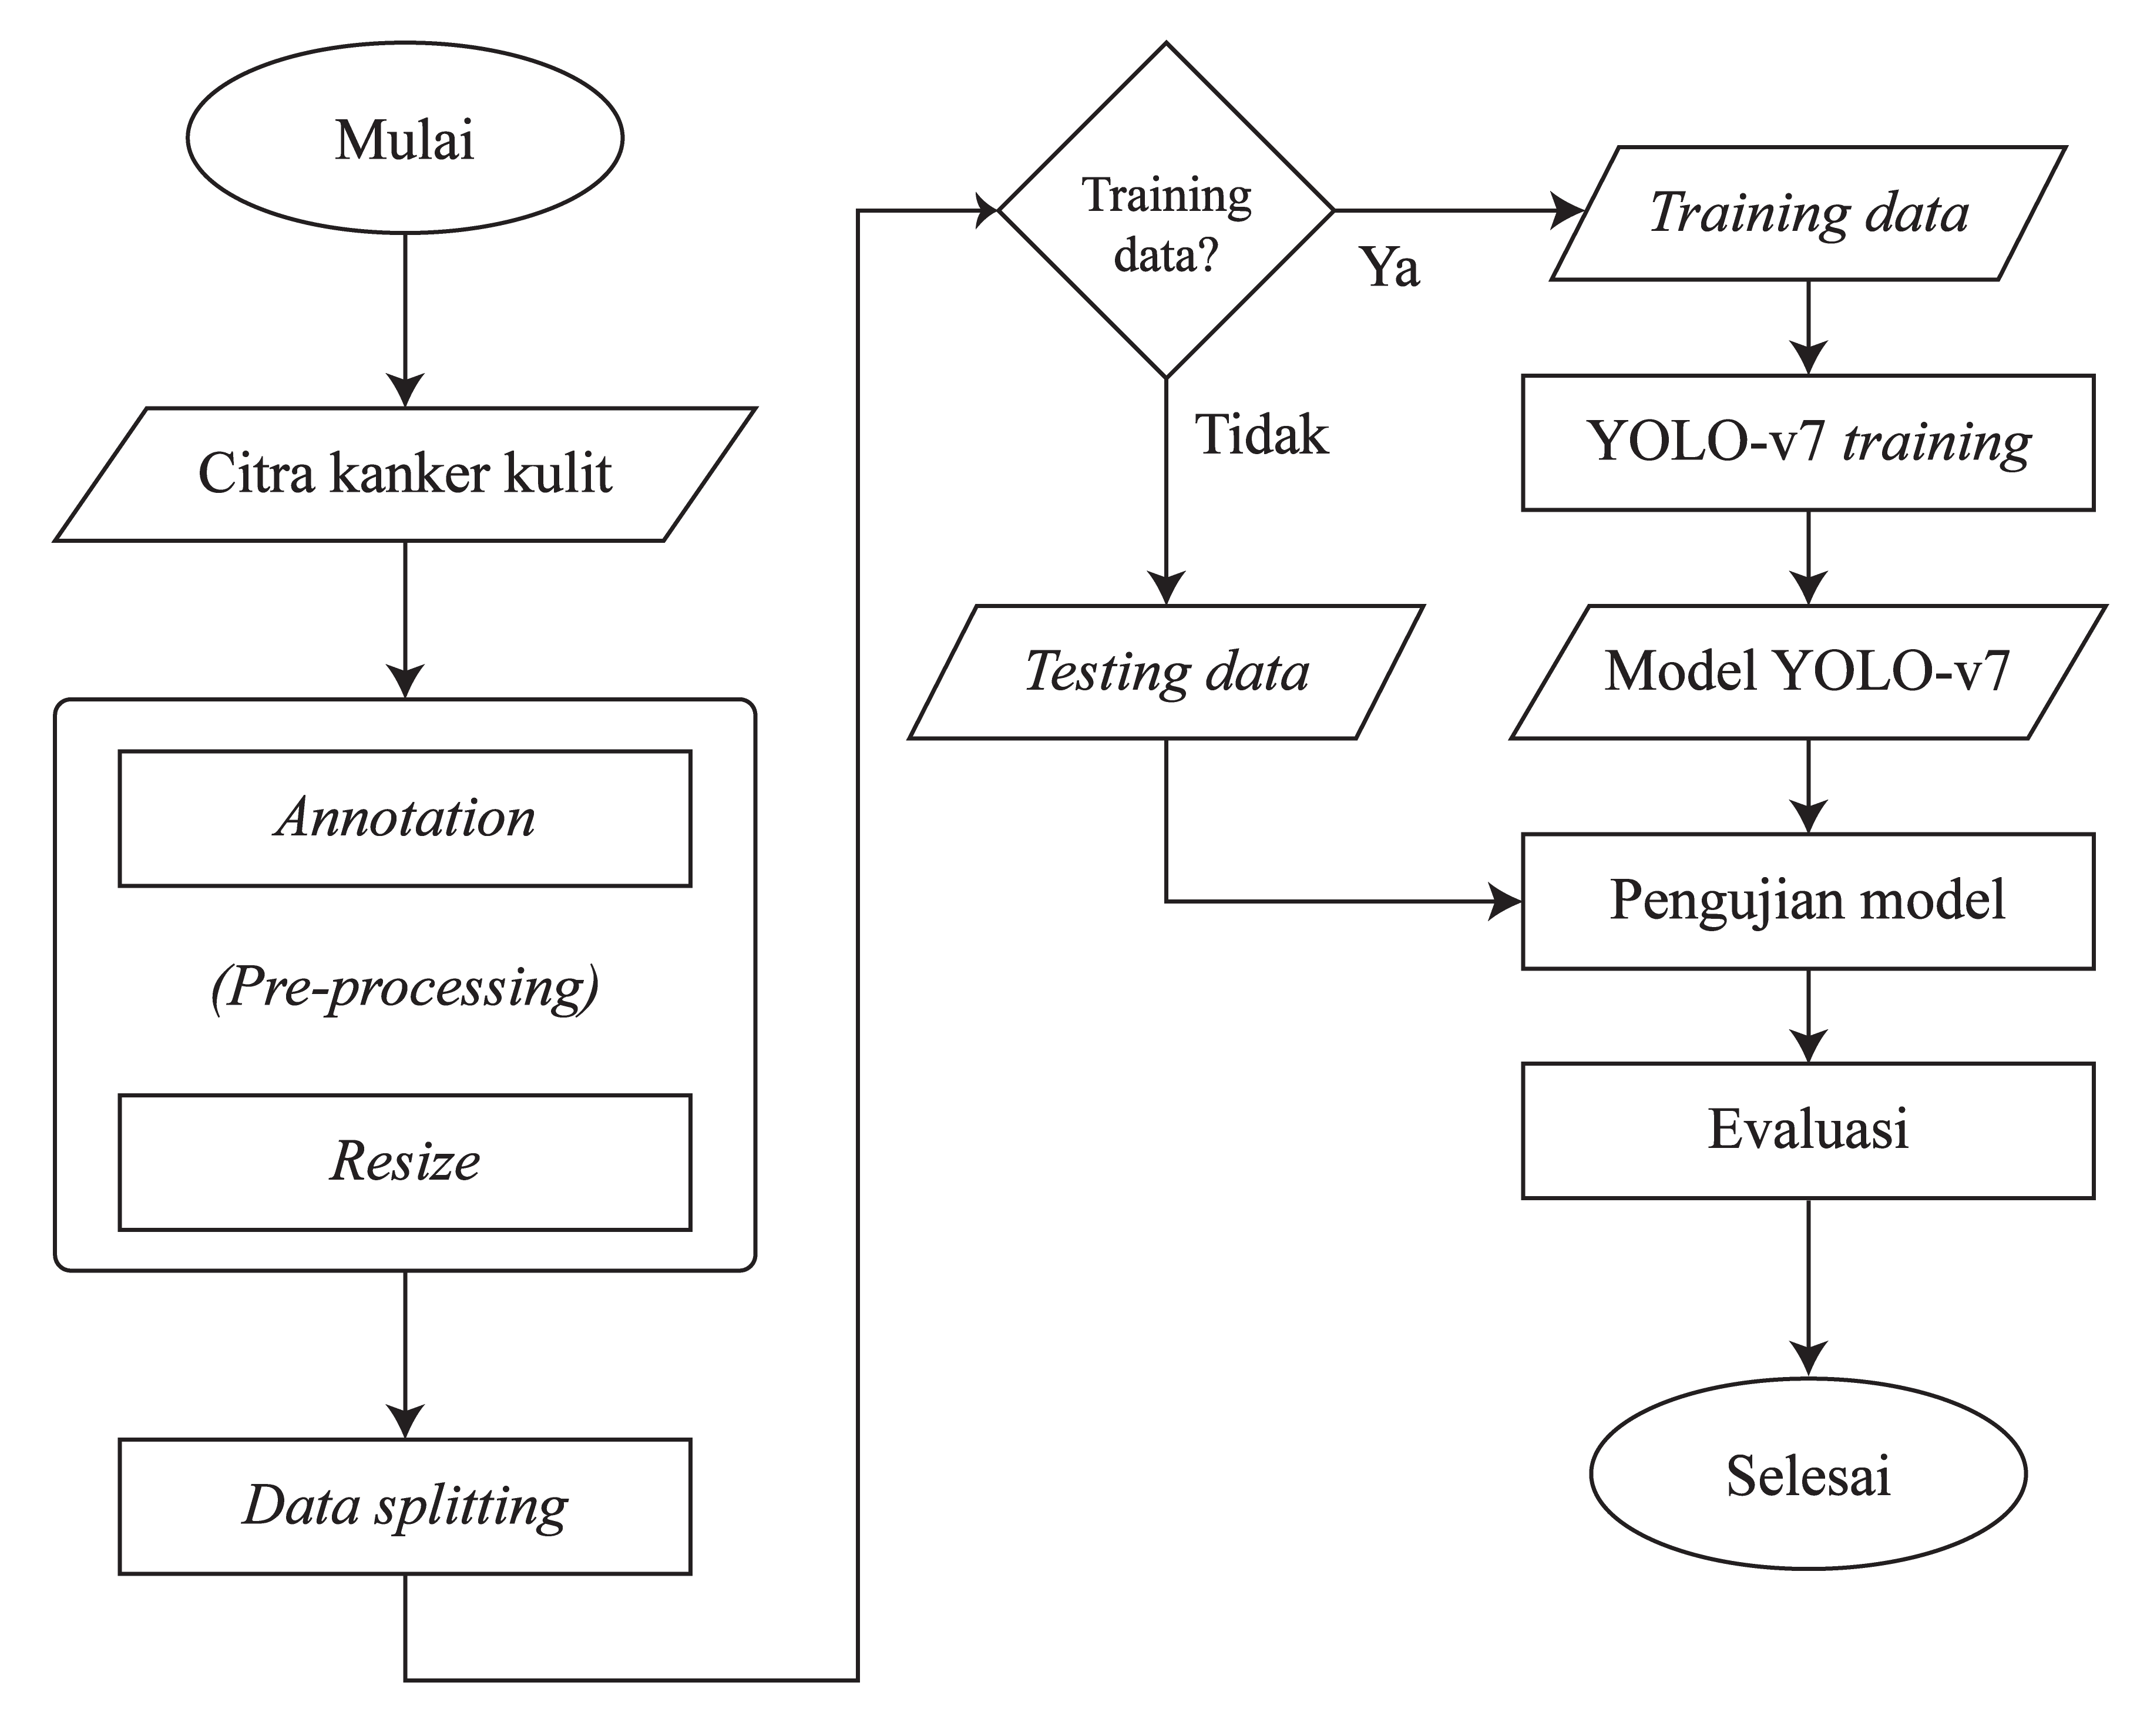
\includegraphics[width=13cm]{../img/Flowchart.png}
        \caption{Diagram alir pada penelitian ini}
        \label{fig:flowchart}
    \end{center}
\end{figure}

Penelitian ini terdiri dari beberapa proses sebagai berikut:
\begin{enumerate}
    \item Tahap \textit{pre-processing} terdiri dari \textit{annotation} dan \textit{resize}. \textit{Annotation} merupakan pemberian kotak pembatas sebuah objek pada sebuah citra. Hal ini dilakukan satu per satu sesuai dengan label yang diberikan dari penyedia dataset, yaitu \textit{ISIC 2019 Challenge}. \textit{Resize} merupakan pengubahan ukuran piksel pada sebuah citra, sehingga penelitian ini melakukan \textit{resize} citra masukan menjadi ukuran $640\times 640$. Rumus \textit{resize} seperti terlihat pada \ref{eq:resize}. Proses \textit{annotation} dan \textit{resize} seperti terlihat pada Gambar \ref{fig:preprocessing}.
    \begin{figure}[H]
        \centering
        \begin{tabular}{ccc}
            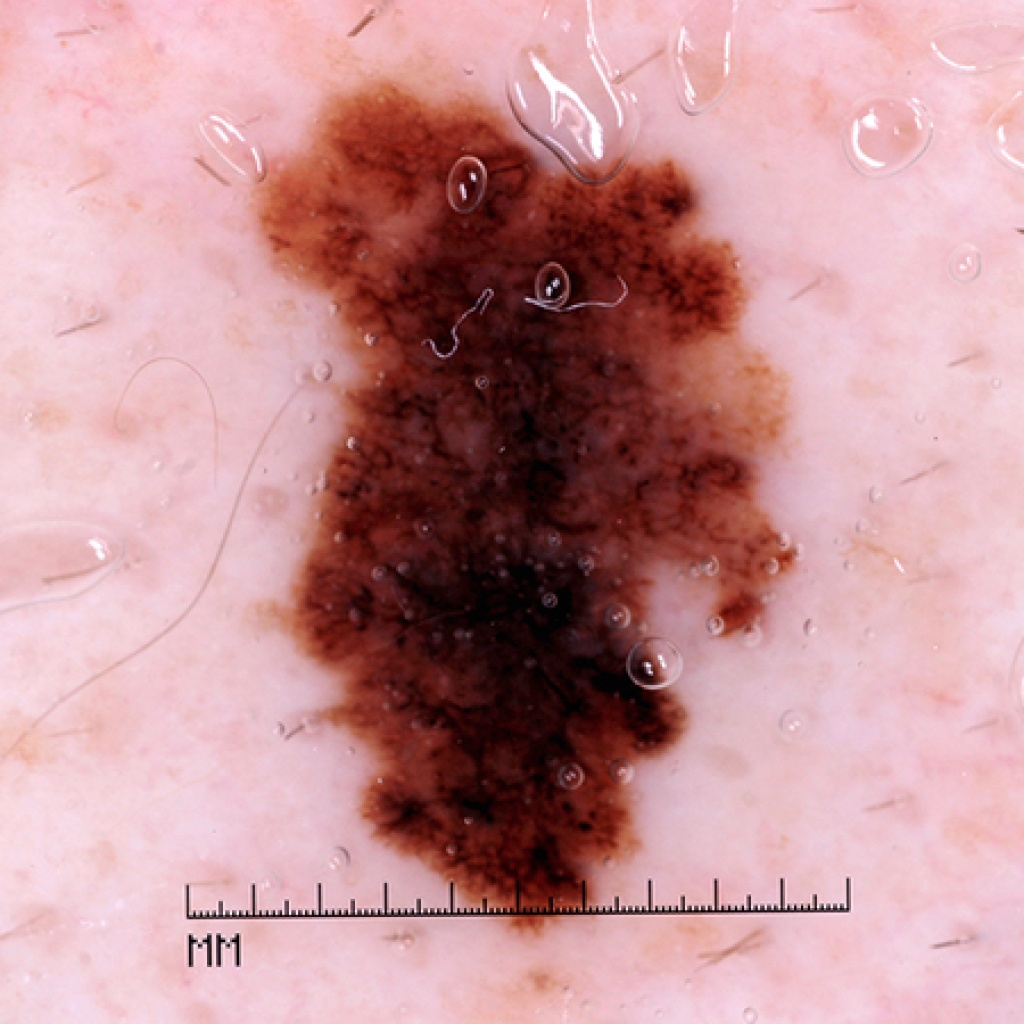
\includegraphics[width=2cm]{../img/bab2/dermoscopy.jpg}
            &
            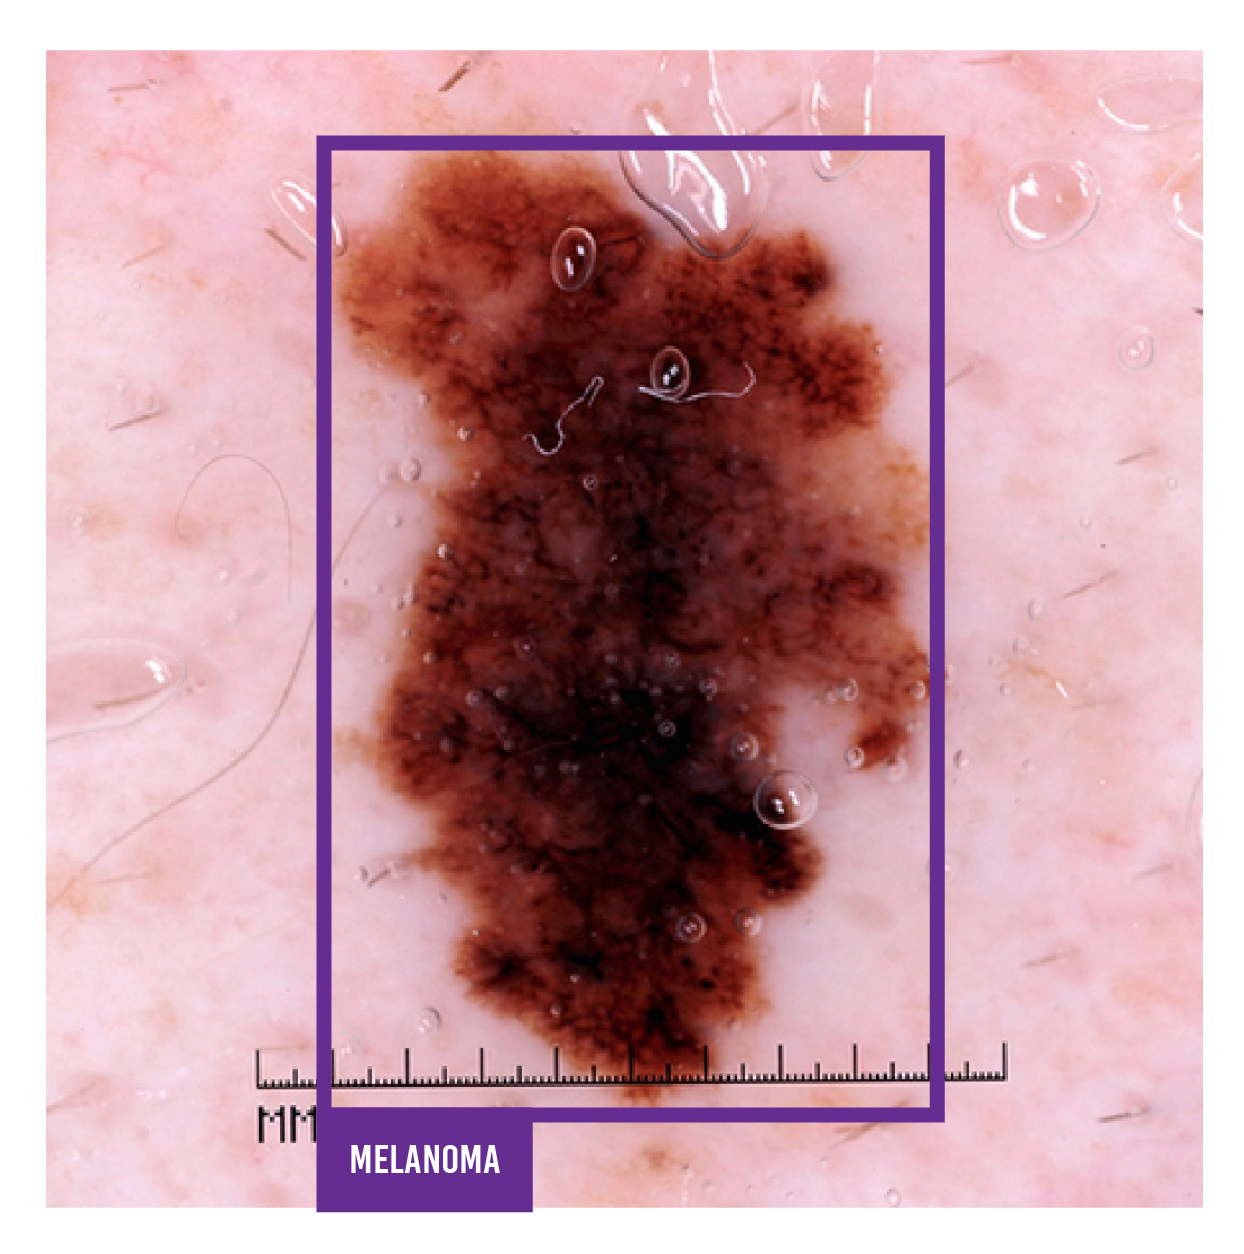
\includegraphics[width=2cm]{../img/Annotation - Latex.png}
            &
            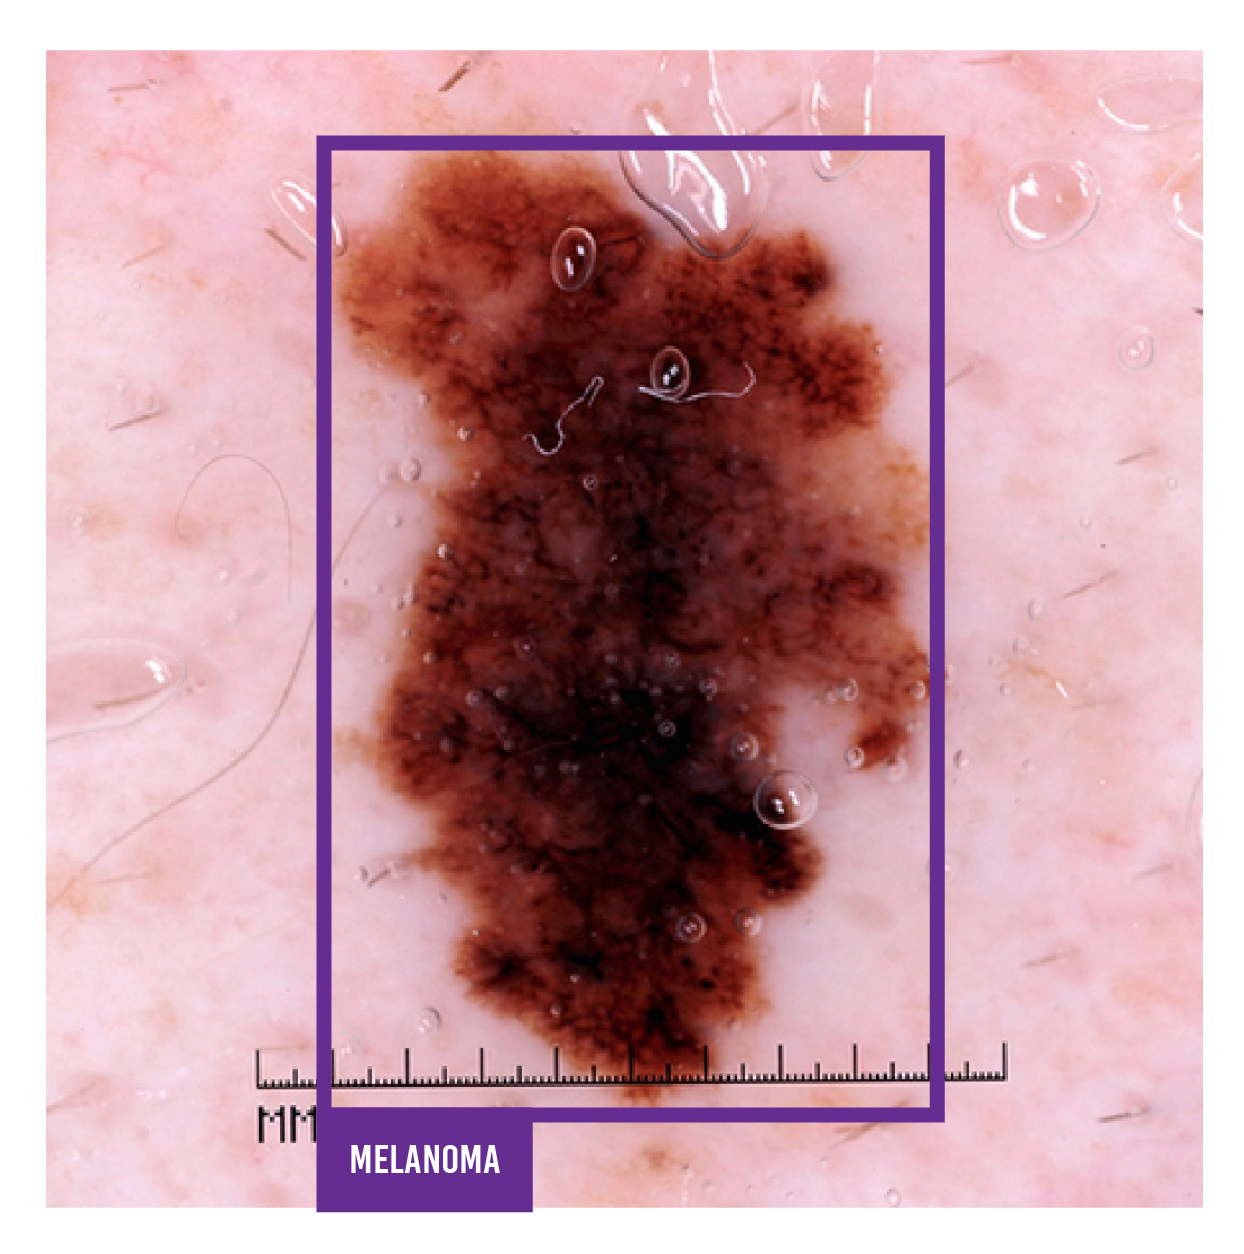
\includegraphics[width=1.5cm]{../img/Annotation - Latex.png}\\
            (a) &(b) &(c)\\
        \end{tabular}
        \caption{Tahap \textit{pre-processing} (a) Citra asli; (b) Citra setelah menerapkan \textit{annotation}; (c) Citra setelah menerapkan \textit{resize}}
        \label{fig:preprocessing}
    \end{figure}

    \item \textit{Data splitting} merupakan tahap pembagian data. Penelitian ini membagi data menjadi tiga, yaitu $70\%$ data untuk proses pelatihan, $20\%$ data untuk proses validasi, dan $10\%$ data untuk proses pengujian.
    \item Proses pembentukan model YOLO-v7 dan YOLO-v7 Tiny berdasarkan uji coba \textit{hyperparameter}. \textit{Hyperparameter} yang digunakan adalah \textit{batch size} dan \textit{epochs}. Nilai \textit{batch size} yang dilakukan uji coba pada penelitian ini adalah $32$, $64$, dan $128$. Sedangkan nilai \textit{epochs} yang dilakukan uji coba pada penelitian ini adalah $300$, $600$, dan $1200$. Proses pembentukan model menggunakan Persamaan \ref{eq:conv-layer} hingga \ref{eq:silu}.
    \item Proses pengujian model yaitu tahap untuk mengetahui tingkat keberhasilan model menggunakan \textit{testing data} untuk mendapatkan hasil evaluasi.
    \item Proses evaluasi menggunakan mAP sehingga dilakukan perhitungan mAP berdasarkan Persamaan \ref{eq:xa1} hingga \ref{eq:map} untuk mendapatkan nilai IoU, \textit{precision}, \textit{recall}, dan mAP.
\end{enumerate}
